%%%%%%%%%%%%%%%%%%%%%%%%%%%%%%%%%%%%%%%%%%%%%%%%%%%%%%%%%%%%%%%%%%%%%%%%%%%%%%%%%%%%%%%%%%%%%%%%
%
% Project CV Written Question Template
%
% This is a LaTeX document. LaTeX is a markup language for producing documents.
% Your task is to answer the questions by filling out this document, then to
% compile this into a PDF document.
%
% TO COMPILE:
% > pdflatex thisfile.tex
%
%
% If you need help with LaTeX, come to office hours. Or, there is plenty of help online:
% https://en.wikibooks.org/wiki/LaTeX
%
% Good luck!
% Prathmesh and the Proj-CV staff
%
%%%%%%%%%%%%%%%%%%%%%%%%%%%%%%%%%%%%%%%%%%%%%%%%%%%%%%%%%%%%%%%%%%%%%%%%%%%%%%%%%%%%%%%%%%%%%%%%
%
% How to include two graphics on the same line:
%
% \includegraphics[width=0.49\linewidth]{yourgraphic1.png}
% \includegraphics[width=0.49\linewidth]{yourgraphic2.png}
%
% How to include equations:
%
% \begin{equation}
% y = mx+c
% \end{equation}
%
%%%%%%%%%%%%%%%%%%%%%%%%%%%%%%%%%%%%%%%%%%%%%%%%%%%%%%%%%%%%%%%%%%%%%%%%%%%%%%%%%%%%%%%%%%%%%%%%

\documentclass[11pt]{article}

\usepackage[english]{babel}
\usepackage[utf8]{inputenc}
\usepackage[colorlinks = true,
            linkcolor = blue,
            urlcolor  = blue]{hyperref}
\usepackage[a4paper,margin=1.5in]{geometry}
\usepackage{stackengine,graphicx}
\usepackage{fancyhdr}
\setlength{\headheight}{15pt}
\usepackage{microtype}
\usepackage{times}
\usepackage[shortlabels]{enumitem}
\setlist[enumerate]{topsep=0pt}
% python code format: https://github.com/olivierverdier/python-latex-highlighting
\usepackage{pythonhighlight}

\frenchspacing
\setlength{\parindent}{0cm} % Default is 15pt.
\setlength{\parskip}{0.3cm plus1mm minus1mm}

\pagestyle{fancy}
\fancyhf{}
\lhead{Prathmesh Madhu\\Project 5 Questions}
\rhead{Project Computer Vision\\
Summer 2021}
\rfoot{\thepage}

\date{}

\title{\vspace{-1cm}Project 5 Questions}


\begin{document}
\maketitle
\thispagestyle{fancy}
\vspace{-3cm}

\section*{Instructions}
\begin{itemize}
  \item 3 questions.
  \item Write code where appropriate; feel free to include images or equations.
  \item \textbf{We do NOT expect you to fill up each page with your answer.} Some answers will only be a few sentences long, and that is okay.
\end{itemize}

\section*{Questions}

%%%%%%%%%%%%%%%%%%%%%%%%%%%%%%%%%%%

\paragraph{Q1:} 

\begin{enumerate} [(a)]
    \item Explain these common terms in machine learning in your words:
    \begin{enumerate} [(i)]
    \item Bias
    \item Variance
    \end{enumerate}
    \item Define these terms in the context of evaluating a classifier:
    \begin{enumerate} [(i)]
    \item Overfitting
    \item Underfitting
    \end{enumerate}
    \item Does bias and variance have any impact on overfitting and underfitting. Can you describe a brief real-world scenario where you can find/observe this?
\end{enumerate}

\emph{Please answer overleaf.}

%%%%%%%%%%%%%%%%%%%%%%%%%%%%%%%%%%%
\pagebreak
\paragraph{A1:} Your answer here.
% Uncomment the stencil below and fill in your solution.

% \begin{enumerate}[(a)]

% \item 
%     \begin{enumerate} [(i)]
%     \item 
%     \item
%     \end{enumerate}

% \item 
%     \begin{enumerate} [(i)]
%     \item 
%     \item
%     \end{enumerate}
% \item 

% \end{enumerate}


%%%%%%%%%%%%%%%%%%%%%%%%%%%%%%%%%%%

\pagebreak
\paragraph{Q2:} Suppose you had to test the selective search algorithm on an image from pedestrian detection dataset (for example: an image taken from traffic camera as shown below), do you think that selective search algorithm will suggest bounding boxes over person(s). 
\begin{figure}[!h]
	\centering
	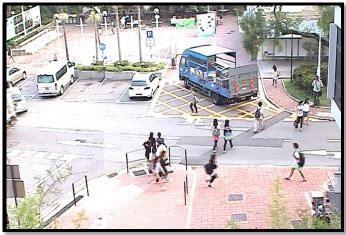
\includegraphics{pedestrian.jpg}
\end{figure}
\begin{enumerate}[(a)]
    \item 
	If yes, what is the justification in your words for this successful behavior of the algorithm? If not, then can you think in which cases does it fail? Can you suggest one way to improve or modify the approach?

    

\end{enumerate}


%%%%%%%%%%%%%%%%%%%%%%%%%%%%%%%%%%%
\paragraph{A2:} Your answer here.
% Uncomment the stencil below and fill in your solution.

% \begin{enumerate}[(a)]

% \item 

% \item 

% \end{enumerate}



%%%%%%%%%%%%%%%%%%%%%%%%%%%%%%%%%%%

\pagebreak
\paragraph{Q3:}
If you were to apply selective search algorithm to detect interesting regions for skin diseases, how do you think the algorithm would have performed? 

\begin{enumerate}[(a)]
\item Which among the four similarity (color, texture, size and shape) do you think contributes more to automatic detection of interesting regions in this case?

\item Combining what you understood so far, what do you think ``objectness" means and do you agree that selective search algorithm inherently finds regions of interest based on ``objectness"?

\end{enumerate}

\emph{Please answer overleaf.}

%%%%%%%%%%%%%%%%%%%%%%%%%%%%%%%%%%%
\pagebreak
\paragraph{A3:} Your answer here.
% Uncomment the stencil below and fill in your solution.

% \begin{enumerate}[(a)]

% \item 

% \item 

% \item 

% \end{enumerate}

%%%%%%%%%%%%%%%%%%%%%%%%%%%%%%%%%%%


%%%%%%%%%%%%%%%%%%%%%%%%%%%%%%%%%%%
\pagebreak
\section*{Feedback? (Optional)}
Please help us make the course better. If you have any feedback for this assignment, we'd love to hear it!


% \pagebreak
% \section*{Any additional pages would go here.}


\end{document}
